\documentclass[11pt,a4paper]{article}

\usepackage[utf8]{inputenc}
\usepackage[T1]{fontenc}
\usepackage[spanish]{babel}
\usepackage{amsmath}
\usepackage{amsfonts}
\usepackage{amssymb}
\usepackage{graphicx}
\usepackage{tabularx}
\usepackage{booktabs}
\usepackage{hyperref}
\usepackage{geometry}
\usepackage{listings}
\usepackage{xcolor}
\usepackage{caption}
\usepackage{subcaption}
\usepackage{titlesec}
\usepackage{parskip}
\usepackage{float}

% Configuración de títulos de párrafos
\titleformat{\paragraph}[hang]
{\normalfont\normalsize\bfseries}{\theparagraph}{1em}{}
\titlespacing*{\paragraph}
{0pt}{3.25ex plus 1ex minus .2ex}{1em}

\geometry{top=3cm, bottom=3cm, left=2.5cm, right=2.5cm}

\hypersetup{
    colorlinks=true,
    linkcolor=black,
    filecolor=magenta,      
    urlcolor=cyan,
}

\definecolor{codegreen}{rgb}{0,0.6,0}
\definecolor{codegray}{rgb}{0.5,0.5,0.5}
\definecolor{codepurple}{rgb}{0.58,0,0.82}
\definecolor{backcolour}{rgb}{0.95,0.95,0.92}

\lstdefinestyle{mystyle}{
    backgroundcolor=\color{backcolour},   
    commentstyle=\color{codegreen},
    keywordstyle=\color{magenta},
    numberstyle=\tiny\color{codegray},
    stringstyle=\color{codepurple},
    basicstyle=\ttfamily\small,
    breakatwhitespace=false,         
    breaklines=true,                 
    captionpos=b,                    
    keepspaces=true,                 
    numbers=left,                    
    numbersep=5pt,                  
    showspaces=false,                
    showstringspaces=false,
    showtabs=false,                  
    tabsize=2
}

\lstset{style=mystyle}

\begin{document}
\begin{titlepage}
    \begin{center}
        \vspace*{1cm}

        \Huge
        \textbf{Guía Práctica 1}

        \vfill

        \Large
        \textbf{Autor:} Simón Saillen

        \Large
        \textbf{Profesores:} Ariel Luis Pola, Pablo Cayuela

        \vspace{0.5cm}

        \Large
        \textbf{Diseño Digital Avanzado}\\
        \vspace{0.2cm}
        \textbf{Fundación Fulgor / FCEFyN}\\
        \vspace{0.2cm}
        Septiembre 2026

    \end{center}
\end{titlepage}
\newpage

\section{Ejercicio 1}

\subsection{Diseño RTL}

Siguiendo el Diseño Digital a nivel RTL de la figura se procedió a implementar
el equivalente en Verilog.

\begin{figure}[H]
    \centering
    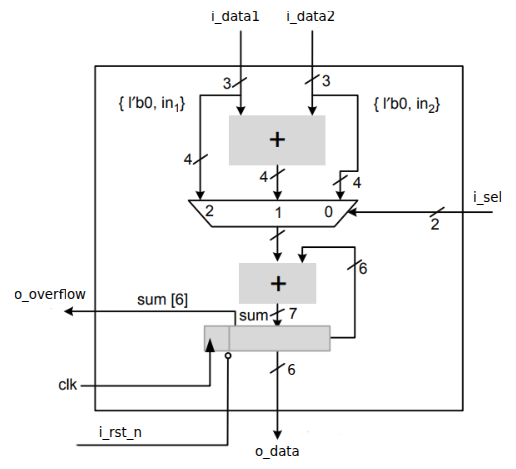
\includegraphics[width=0.5\textwidth]{../images/RTL_Design.png}
    \caption{Diagrama RTL del ejercicio 1.}
\end{figure}

Iniciando con la definicion del modulo y la declaracion de entradas y salidas, se llega al siguiente snippet:

\begin{lstlisting}[language=Verilog]
module E1 (
    input clk, reset_n,
    input [2:0] i_data1, i_data2,
    input [1:0] i_sel,
    output wire [5:0] o_data,
    output wire o_overflow
);
\end{lstlisting}

A simple vista se puede observar que el diseño constara de dos partes, una parte
combinacional y otra secuencial. La parte combinacional se encarga del multiplexado
de las entradas, se implemento de la siguiente manera:

\begin{lstlisting}[language=Verilog]
    reg [3:0] mux_exit;

    always @(*) begin
        case (i_sel)
            2'b00: mux_exit = {1'b0, i_data2};
            2'b01: mux_exit = i_data1 + i_data2;
            2'b10: mux_exit = {1'b0, i_data1};
            default: mux_exit = 4'b0000;
        endcase
    end
\end{lstlisting}

La parte secuencial se encarga de, utilizando la salida del multiplexor, realizar
la suma de retroalimentacion y detectar el overflow, esto se implemento de la siguiente manera:

\begin{lstlisting}[language=Verilog]
    reg [6:0] sum;

    always @(posedge clk, negedge reset_n) begin
        sum <= (~reset_n) ? 0 : mux_exit + sum[5:0];
    end

    assign o_overflow = sum[6];
    assign o_data = sum[5:0];

endmodule
\end{lstlisting}

Para verificar si se logro realizar una equivalencia entre el diseño RTL
y el diseño en Verilog, usando Vivado se sintetizo y se obtuvo el siguiente \textit{Elaborated Design}:

\begin{figure}[H]
    \centering
    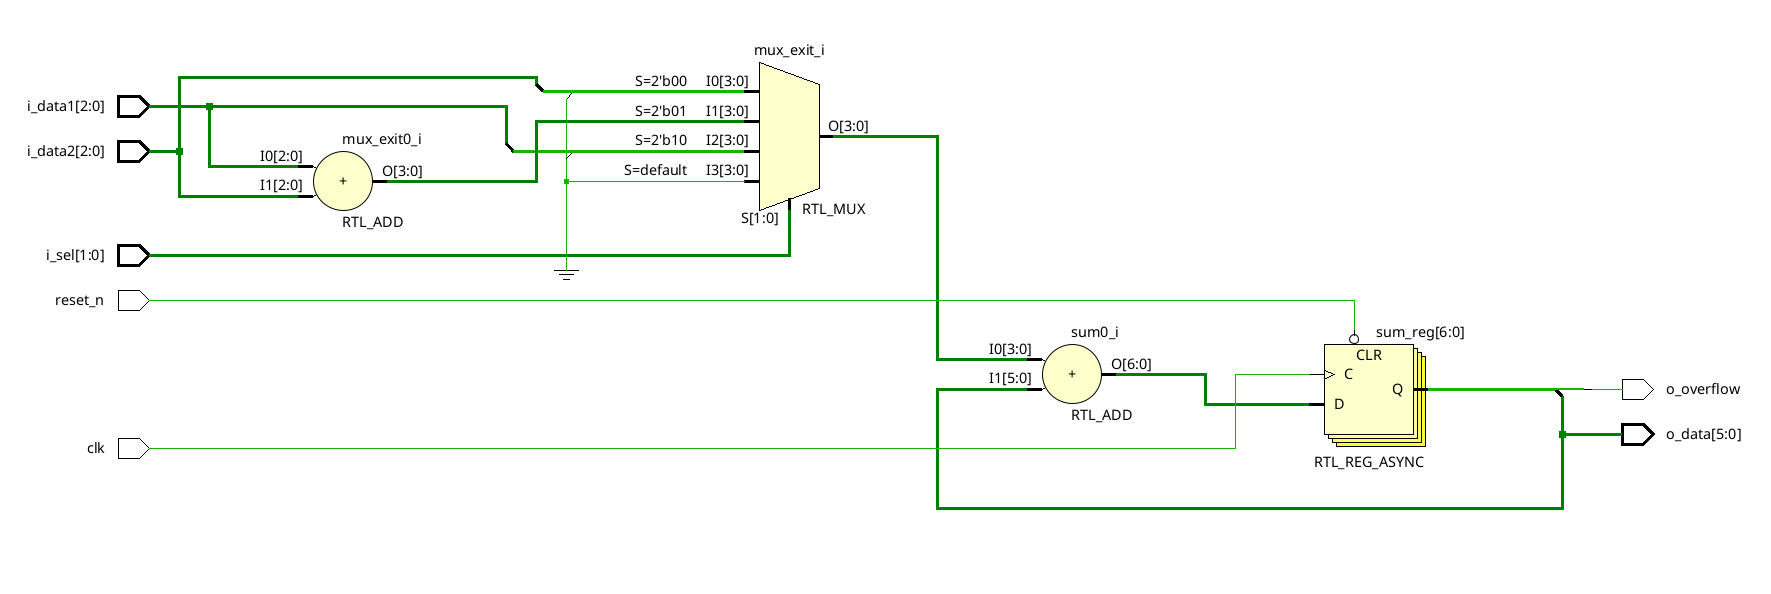
\includegraphics[width=0.9\textwidth]{../images/Elaborated_Design.png}
    \caption{Diagrama de diseño elaborado del ejercicio 1.}
\end{figure}

Se puede comprobar que el diseño sintetizado si es equivalente al diseño RTL.

\subsection{Testbench}

Para verificar el correcto funcionamiento del diseño, se procedió a realizar un testbench
que simule el comportamiento del mismo.

El testbench se implementó siguiendo los siguientes pasos:

\begin{enumerate}
    \item Se definieron las señales de entrada y salida del módulo a probar.
    \item Se definió un modelo de referencia para comparar los resultados obtenidos con los esperados.
    \item Se generaron casos de prueba que cubran todas las posibles combinaciones de entradas
          y condiciones de operación.*
    \item Se genero un test para calcular los ciclos de reloj necesarios para el overflow.**
\end{enumerate}

(*): Los casos de prueba consistieron en un barrido sistematico de los valores de \texttt{i\_sel}, utilizando
valores aleatorios para \texttt{i\_data1} y \texttt{i\_data2}, y verificando que la
salida del diseño coincidiera con la salida del modelo de referencia. El modelo de referencia sigue el valor
esperado teorico en base a las operaciones realizadas.

(**): El test para calcular los ciclos de reloj necesarios para el overflow
consistió en alimentar al diseño con valores iniciales y contar los ciclos de
reloj hasta que se produjera el overflow.

Al correr el testbench, se obtuvieron los siguientes resultados:

\begin{figure}[H]
    \centering
    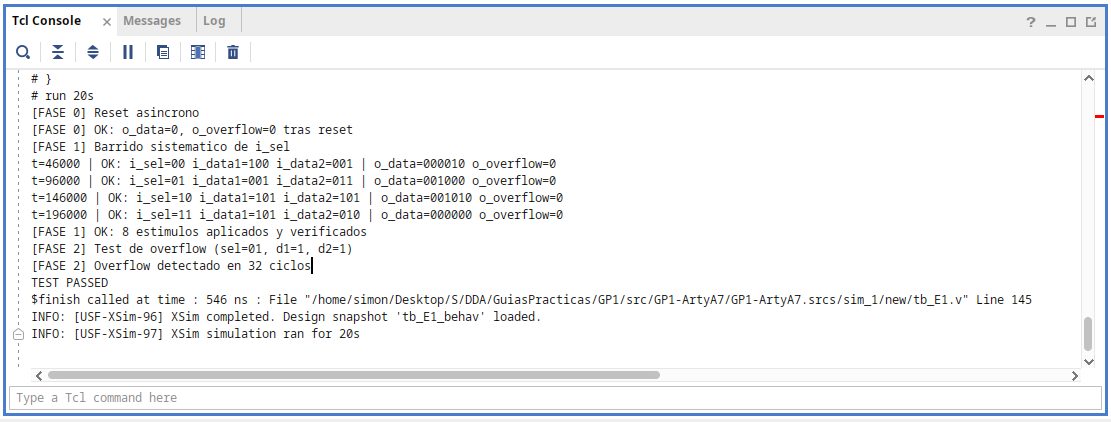
\includegraphics[width=0.9\textwidth]{../images/Testbench1.png}
    \caption{Resultados del testbench del ejercicio 1.}
\end{figure}

El resultado de overflow se obtuvo en 32 ciclos de iteracion, lo cual coincide con el valor esperado teorico,
esto se puede comprobar con la siguiente ecuacion:

\begin{figure}[H]
    $y_0: (1 + 1) + 0$\\
    $y_1: (1 + 1) + 2$\\
    $y_2: (1 + 1) + 4$\\
    $y_i: 2 + (y_{i-1})$\\
    overflow en $2^5 + 1 = 33$\\
    $33: 2 + (y_{i-1}) \rightarrow y_{i-1} = 33 - 2 = 31$\\
    $y_{32} = 2 + (y_{31})\rightarrow\text{overflow}$
\end{figure}

\section{Ejercicio 2}

Las operaciones a interpretar en un esquematico son las siguientes:

\begin{lstlisting}[]
    o_dataC = i_dataA + i_dataB
    o_dataC = i_dataA - i_dataB
    o_dataC = i_dataA & i_dataB
    o_dataC = i_dataA | i_dataB
\end{lstlisting}

Con \texttt{o\_dataC}, \texttt{i\_dataA} y \texttt{i\_dataB} de 16 bits, y un selector de 2 bits \texttt{i\_sel}.

A simple vista se puede observar que el diseño se corresponde a un multiplexor
de 4 entradas y 1 salida, con un selector de 2 bits. El diseño se implemento de la siguiente manera:

\begin{figure}[H]
    \centering
    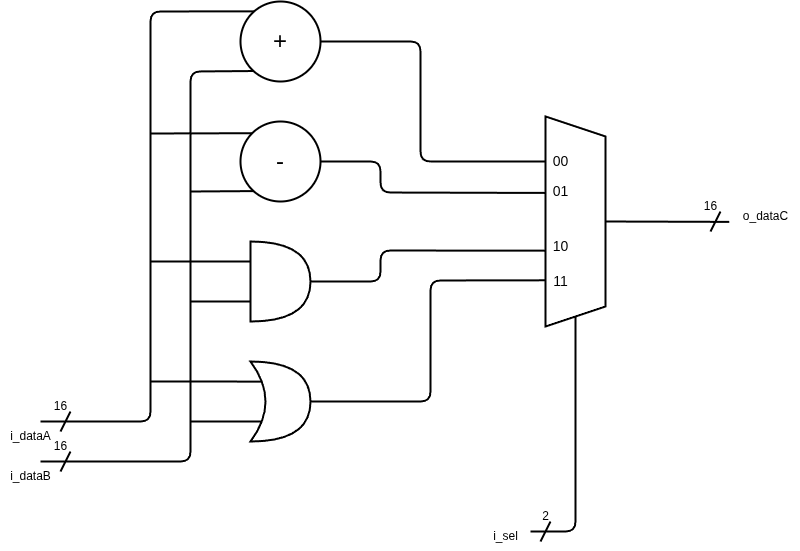
\includegraphics[width=0.8\textwidth]{../images/E2_Design.drawio.png}
    \caption{Esquematico del ejercicio 2.}
\end{figure}

El codigo Verilog correspondiente es bastante sencillo, y se implemento de la siguiente manera:

\begin{lstlisting}[language=Verilog]
module E2 (
    input [15:0] i_dataA, i_dataB,
    input [1:0] i_sel,
    output reg [15:0] o_dataC
);

    always @(*) begin
        case (i_sel)
            2'b00: o_dataC = i_dataA + i_dataB;
            2'b01: o_dataC = i_dataA - i_dataB;
            2'b10: o_dataC = i_dataA & i_dataB;
            2'b11: o_dataC = i_dataA | i_dataB;
            default: o_dataC = 16'b0;
        endcase
    end

endmodule
\end{lstlisting}

Esto se puede comprobar sintetizando el diseño en Vivado y obteniendo el \textit{Elaborated Design}:

\begin{figure}[H]
    \centering
    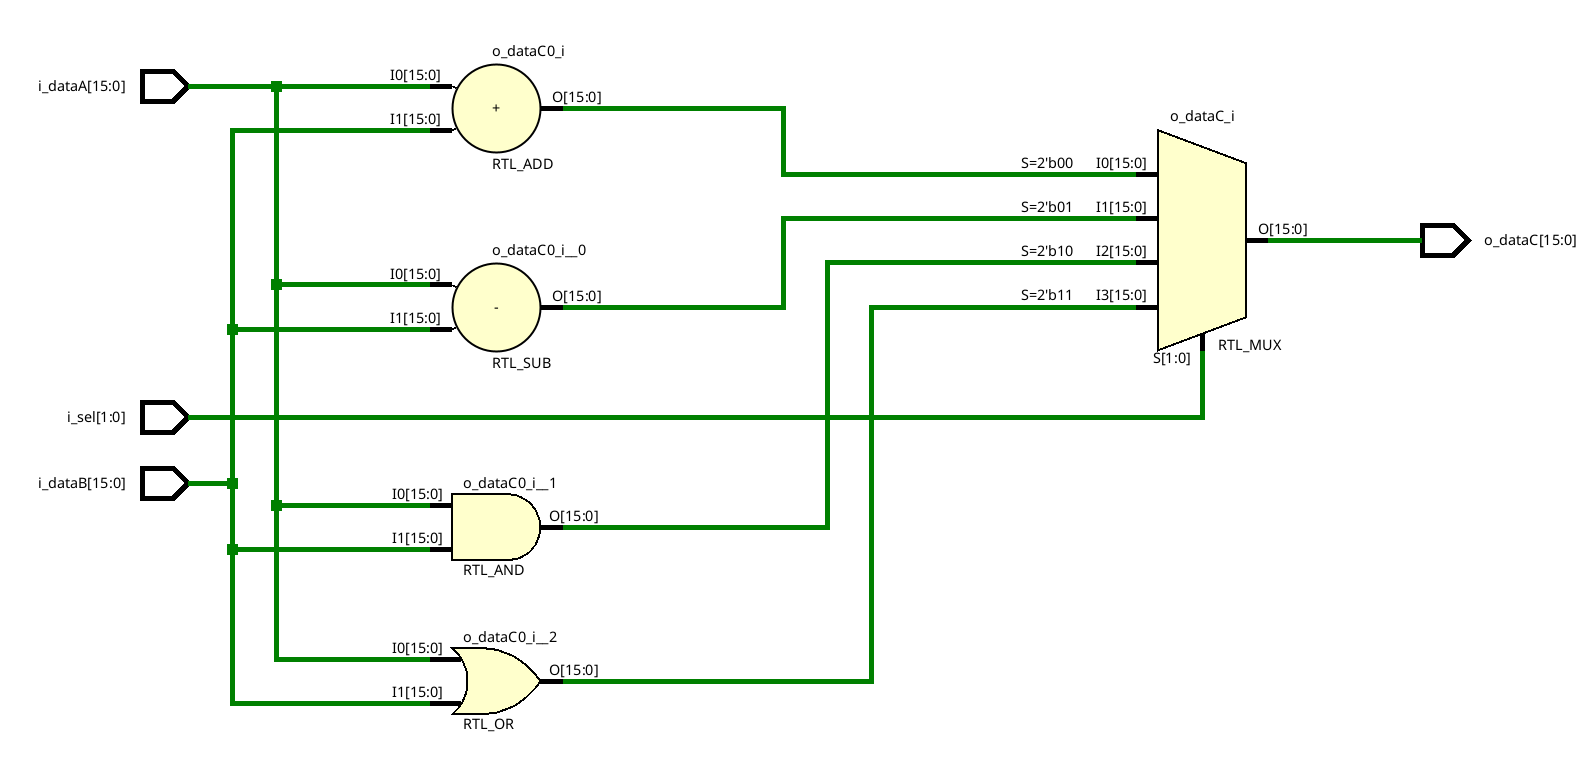
\includegraphics[width=0.9\textwidth]{../images/E2_Elaborated_Design.png}
    \caption{Diagrama de diseño elaborado del ejercicio 2.}
\end{figure}

El testbench se implemento de la misma manera que el ejercicio 1, generando casos de prueba
para cada una de las operaciones utilizando numeros aleatorios, y comparando los resultados
obtenidos con los esperados. Estos fueron los resultados obtenidos:

\begin{figure}[H]
    \centering
    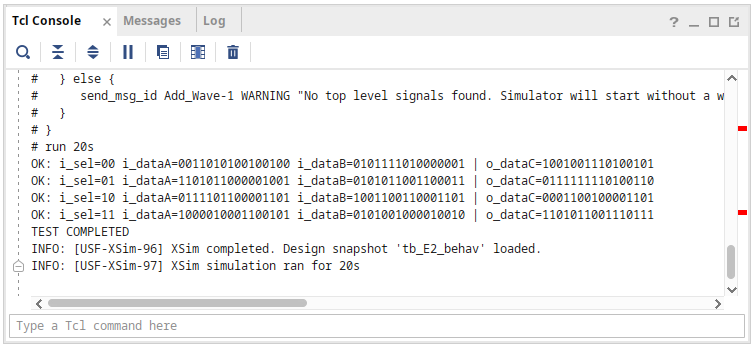
\includegraphics[width=0.9\textwidth]{../images/Testbench2.png}
    \caption{Resultados del testbench del ejercicio 2.}
\end{figure}

\section{Ejercicio 3}

\begin{figure}[H]
    \centering
    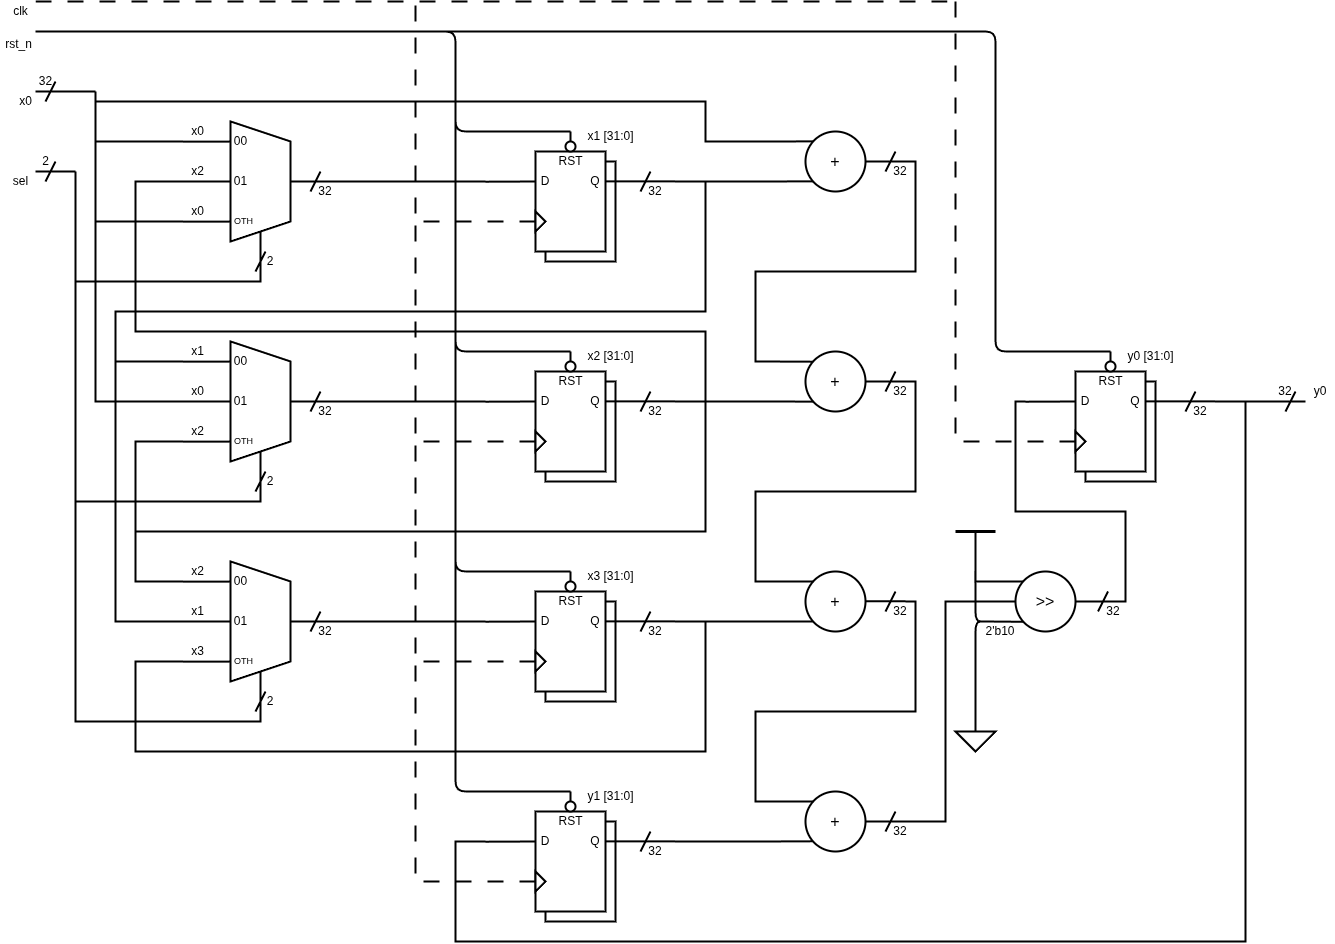
\includegraphics[width=0.9\textwidth]{../images/E3_Design.drawio.png}
    \caption{Esquematico del ejercicio 3.}
\end{figure}

\section{Ejercicio 4}

\subsection{Cálculo de Bits de Salida}

Para determinar la cantidad de bits necesarios para la salida con \textit{full-resolution} (sin perdidas
por desbordamiento ni truncamiento), se debe analizar la ecuacion diferencial y la resolucion de entrada.

El rango dinamico de la entrada es de 8 bits, lo que significa que los valores de entrada pueden
variar entre 0 y 255. La ecuacion diferencial tiene terminos que suman y restan valores de entrada y salida,
lo que puede llevar a un aumento en el rango de valores posibles para la salida.

Para el analisis se separan los terminos de la ecuacion diferencial en dos partes: los terminos de entrada
y los terminos de salida.

\textbf{Terminos de entrada:}

- \textbf{Maximo Valor:} Si todas las entradas son 255 (menos \texttt{x[n-1]} ya que resta), el resultado
de los terminos de entrada seria:
\begin{equation}
    255 - 0 + 255 + 255 = 765
\end{equation}
- \textbf{Minimo Valor:} Si todas las entradas son 0 (y \texttt{x[n-1] = 255}), el resultado de los
terminos de entrada seria:
\begin{equation}
    0 - 255 + 0 + 0 = -255
\end{equation}

Entonces el rango de valores posibles para los terminos de entrada es de -255 a 765.

\textbf{Terminos de salida:}

Para los terminos de salida, se tiene que \texttt{y[n-1]} y \texttt{y[n-2]} son valores de salida realimentados,
por lo que su valor maximo y minimo depende del valor maximo y minimo de la salida.

Usando la ecuacion de lazo cerrado, se puede determinar el valor maximo y minimo de la salida tomando
en cuenta los valores maximos y minimos de los terminos de entrada y utilizando la mayor ganancia posible.

La ecuacion de lazo cerrado es:
\begin{equation}
    Y[n] = \frac{x[n]_{max/min}}{1 - 0.5 - 0.25} = \frac{x[n]_{max/min}}{0.25}
\end{equation}

- \textbf{Maximo Valor:} Equivale al caso en que todas las entradas son 255 (menos \texttt{x[n-1]}):
\begin{equation}
    Y[n]_{max} = \frac{765}{1 - 0.5 - 0.25} = \frac{765}{0.25} = 3060
\end{equation}

- \textbf{Minimo Valor:} Equivale al caso en que todas las entradas son 0 (y \texttt{x[n-1] = 255}):
\begin{equation}
    Y[n]_{min} = \frac{-255}{1 - 0.5 - 0.25} = \frac{-255}{0.25} = -1020
\end{equation}

Entonces el rango de valores posibles para la salida es de -1020 a 3060.

Con \texttt{12 bits}, se puede representar valores de -2048 a 2047, lo cual no es suficiente para cubrir el
rango de salida. Con \texttt{13 bits}, se puede representar valores de -4096 a 4095 lo cual si es suficiente para
cubrir el rango de salida.

En conclusion, se necesitan \textbf{13 bits} para la salida con full-resolution.

\subsection{Arquitectura de la ecuacion diferencial}

\begin{figure}[H]
    \centering
    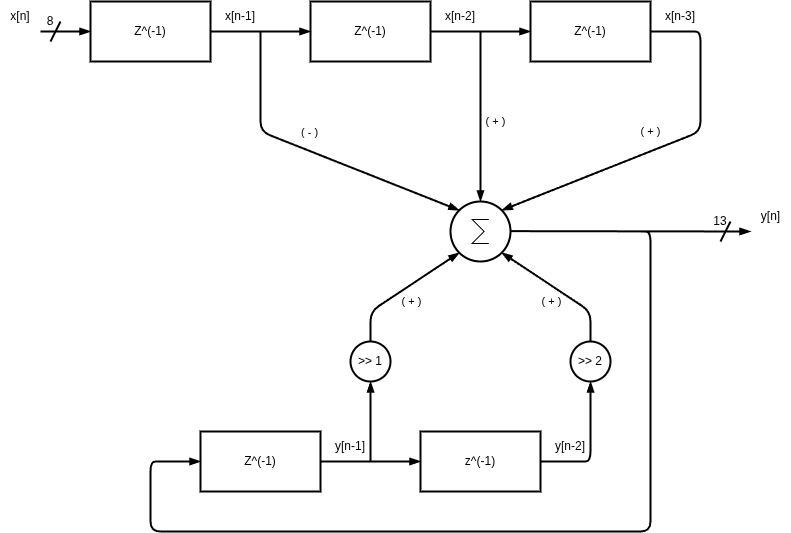
\includegraphics[width=0.9\textwidth]{../images/E4_ArqDesign.drawio.png}
    \caption{Diagrama de bloques del ejercicio 4.}
\end{figure}

\subsection{Diseño RTL}

La ecuacion diferencial a representar es la siguiente:

\begin{equation}
    y[n] = x[n] - x[n-1] + x[n-2] + x[n-3] + 0.5y[n-1] + 0.25y[n-2]
\end{equation}

En el caso de las multiplicaciones, la primera se puede interpretar como dividir el valor por 2 y
la segunda como dividir el valor por 4, esto se puede implementar de manera sencilla con desplazamientos
a la derecha.

Quedando asi la ecuacion a implementar en Verilog:

\begin{lstlisting}[language=Verilog]
  y[n] = x[n] - x[n-1] + x[n-2] + x[n-3] + y[n-1] >> 1 + y[n-2] >> 2;
\end{lstlisting}

Los valores de muestras \textit{pasadas} se pueden almacenar en registros internos, luego mediante
bloques secuenciales se puede ir actualizando el valor de las muestras, y finalmente se puede
implementar la ecuacion en un bloque combinacional.

\newpage

Luego de analizar la ecuacion y el diagrama de bloques, se implemento el siguiente codigo Verilog:

\begin{lstlisting}[language=Verilog]
module E4 (
    input clk, rst_n,
    input [7:0] x,
    output [12:0] y
);

    reg [12:0] x1, x2, x3;
    reg [12:0] y1, y2;
    
    assign y = {5'b0, x} - x1 + x2 + x3 + (y1 >> 1) + (y2 >> 2);

    always @(posedge clk or negedge rst_n) begin
        if (~rst_n) begin
            { x1, x2, x3 } = { 13'b0, 13'b0, 13'b0 };
            { y1, y2 } = { 13'b0, 13'b0 };
        end
        else begin
            { x1, x2, x3 } = { {5'b0, x}, x1, x2 };
            { y1, y2 } = { y, y1 };
        end
    end

endmodule
\end{lstlisting}

\subsection{Testbench}

El testbench para este ejercicio se implemento de manera similar a los anteriores, generando casos de
prueba aleatorios y comparando los resultados obtenidos con los esperados.

El testbench se implemento de la siguiente manera:

\begin{itemize}
    \item Se definieron las señales de entrada y salida del módulo a probar.
    \item Se definieron registros internos para almacenar las muestras pasadas de entrada y salida. Estos
          registros se actualizaron en cada ciclo de reloj.
    \item Se generan valores aleatorios para la entrada \texttt{x} y se calcula el valor esperado de
          la salida \texttt{y} utilizando la ecuacion diferencial.
    \item Se comparan los valores obtenidos de la salida \texttt{y} con los valores esperados y se
          muestran los resultados en la consola.
\end{itemize}

Luego de correr el testbench, se obtuvieron los siguientes resultados:

\begin{figure}[H]
    \centering
    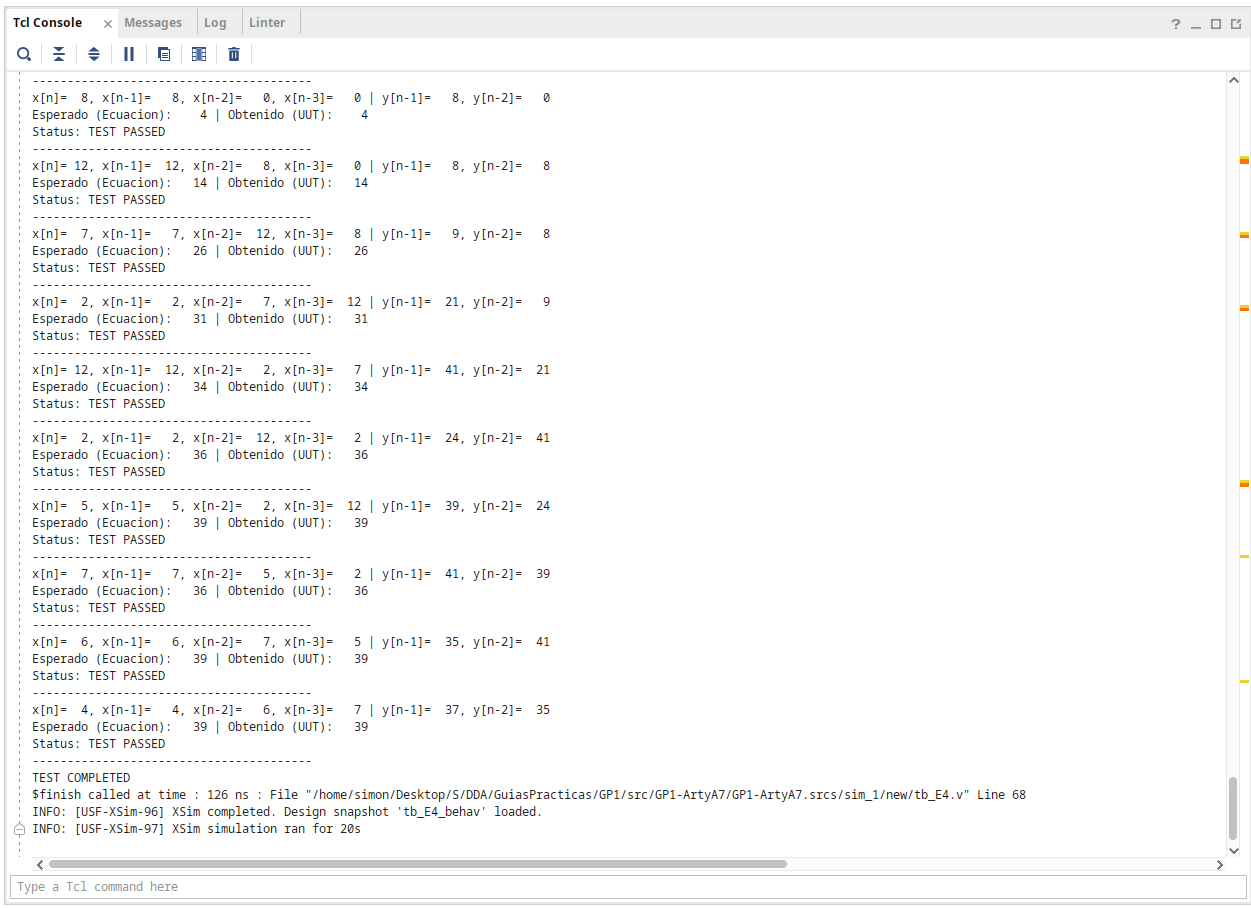
\includegraphics[width=0.9\textwidth]{../images/Testbench4.png}
    \caption{Resultados del testbench del ejercicio 4.}
\end{figure}

\end{document}